\documentclass[11pt,a4paper]{article}
\usepackage{fontspec}
\setmainfont{TeX Gyre Pagella}
\newfontfamily\headfont{Inter}[UprightFont=*-ExtraBold,BoldFont=*-ExtraBold,Extension=.otf,Path=/usr/share/fonts/opentype/inter/]
\usepackage[a4paper,margin=2.3cm]{geometry}
\usepackage{graphicx,booktabs,float,caption,array,xcolor,longtable}
\usepackage{xurl}
\usepackage[hidelinks]{hyperref}
\usepackage{titlesec}
\usepackage[round]{natbib}
\usepackage{setspace}
\setstretch{1.05}
\renewcommand{\topfraction}{0.9}
\renewcommand{\bottomfraction}{0.8}
\renewcommand{\textfraction}{0.1}
\renewcommand{\floatpagefraction}{0.75}
\setlength{\parindent}{0pt}
\setlength{\parskip}{0.55em}
\titleformat{\section}{\headfont\Large}{\thesection}{0.8em}{}
\titleformat{\subsection}{\headfont\large}{\thesubsection}{0.8em}{}
\captionsetup{font=small,labelfont=bf}
\urlstyle{same}
\hypersetup{pdftitle={Which Way Do the UK's Churches Face?},pdfauthor={Tristan Hotham}}

\begin{document}
\begin{center}
{\Large\bfseries Which Way Do the UK's Churches Face?\par}
\vspace{0.4em}
{\large The axes of 32,007 church footprints from OpenStreetMap,\\and a test of the patron saint's sunrise\par}
\vspace{1.2em}
{\large Tristan Hotham\par}
\vspace{0.3em}
{\small Independent researcher\\
ORCID: 0000-0003-4931-9349\\
DOI: \href{https://doi.org/10.5281/zenodo.24052501}{10.5281/zenodo.24052501}\par}
\vspace{0.8em}
2026
\end{center}

\begin{quote}
\small
\begin{center}\textbf{Abstract}\end{center}
Christian churches are traditionally built facing east, but most turn a few degrees from it, and a long-standing explanation holds that the line was set towards sunrise on the patron saint's feast day. I measure the long axis of every church footprint in OpenStreetMap for the United Kingdom that is clearly longer than it is wide (32,007 buildings), as the long side of the minimum-area enclosing rectangle in a local true-north frame, and join saints, dates and listing grades from Wikidata. 30.4\% of all churches lie within 10° of due east, but 53.5\% of the historic parish churches (dated before 1540, or undated and listed Grade I, II* or category A), against 24.9\% of churches dated 1800 to 1913, 19.9\% of those from 1914 and 14.2\% of Free Church chapels (11.1\% would be expected by chance). The patron saint's day explains nothing: across 5,687 historic churches with a fixed-feast saint, the mean absolute difference between axis and feast-day sunrise (30.9°, with Julian-calendar dates for medieval foundations) is no smaller than when the saints are shuffled at random (30.9°, permutation p = 0.54); churches of midsummer and midwinter saints point the same way (85.5° and 85.4°) although their feast-day sunrises differ by 78.3°. Historic churches lean north of east by 4.9° on average, more in the west of England and Wales than in the east. In towns, churches built from 1800 onwards follow the local street grid more often than east.

\textbf{Keywords:} church orientation; archaeoastronomy; OpenStreetMap; Wikidata; patron saints; medieval churches; urban form
\end{quote}

\section{Introduction}
Orientation, the setting of a church with its altar to the east, is one of the most widespread conventions of Christian building. Yet the axes of English parish churches rarely point exactly east. Since the nineteenth century a popular explanation has been that the builders laid out the axis at dawn on the day of the church's patron saint, so that a church of a midsummer saint would turn north of east and one of a midwinter saint south of it. \citet{alicunich} measured 143 major churches built between the mid eleventh and late twelfth centuries; they found no support for alignment by magnetic compass and concluded that the patron-saint sunrise could account for up to 43\% of their sample if sunrise and sunset are both allowed. \citet{hinton} surveyed about 1,500 rural churches and found that churches of summer and winter saints face in the same directions, with a difference in mean alignment of about 10° between the west and east of England. \citet{furuhashi} measured entrance bearings of 114 churches in Milan from OpenStreetMap and found a westward tendency (the entrance opposite an eastern altar) moderated by the urban fabric.

OpenStreetMap now holds the outlines of tens of thousands of church buildings in the United Kingdom, and Wikidata links many of them to their patron saint, date and heritage listing. This allows the question to be asked of almost every church at once, with a test that does not depend on choosing a sample: does knowing the saint help to predict the axis? The study also asks how much churches vary, whether older churches differ from Victorian and modern ones and between denominations, and whether the street grid is a better guide in towns. It accompanies an interactive map of every measured church (\url{https://maps.tristanhotham.com/church-orientation/}).

\section{Data}
\textbf{Footprints.} Every OpenStreetMap \citep{osm} element in the United Kingdom tagged \texttt{building=church}, \texttt{cathedral} or \texttt{chapel} (27,560 polygons), and every element tagged \texttt{amenity=place\_of\_worship} with \texttt{religion=christian} drawn as another kind of building (13,076 polygons), was extracted with the QLever SPARQL engine \citep{qlever} over osm2rdf, with name, dedication, denomination, heritage, start date and Wikidata tags. Elements mapped only as points were dropped, since they have no shape. Footprints tagged as houses, schools, offices and similar (265) and footprints lying inside a larger church footprint (47, such as a chapel mapped within a cathedral) were removed.

\textbf{Wikidata.} Wikidata \citep{wikidata} items for church buildings in the United Kingdom give the dedication (P825), inception (P571), heritage designation (P1435) and OpenStreetMap way identifier (P10689). Items were joined to footprints through the OpenStreetMap \texttt{wikidata} tag, then through P10689, then by the item's coordinates lying inside a footprint (or within about 15 m of exactly one); a footprint claimed by two items was left unjoined. 21,956 of the measured footprints are joined. Wikidata's dedications to Oswald of Worcester were reassigned to Oswald of Northumbria (feast 5 August), since almost all are northern St Oswald churches. Listing grades come from Historic England, Cadw, Historic Environment Scotland and the Northern Ireland record through Wikidata.

\textbf{Saints and feasts.} The dedication is taken from Wikidata where present, otherwise from the OpenStreetMap dedication tag or the name, parsed with the dedication parser of the saints-geography study \citep{saintsgeo}; 18,610 measured churches have one. Feast days for 69 saints and dedications with a single fixed principal feast were taken from the standard Western calendars (for example 24 June for John the Baptist, 29 June for Peter, 29 September for Michael, 1 November for All Saints, 30 November for Andrew, 6 December for Nicholas and 21 December, the traditional date, for Thomas the Apostle); they are listed in the code. Dedications without one fixed feast (the Holy Trinity, Christ, the Holy Cross, Paul alone, John without a qualifier, and Mary, who is treated separately) are left out of the feast test.

\section{Methods}
\subsection{The axis}
Each footprint (the largest polygon of a multipolygon) is projected to a local equirectangular frame about its own centroid, which keeps true north up and distorts lengths by much less than a metre over a building. The minimum-area enclosing rectangle \citep{freeman} gives the axis: the bearing of its long side, folded into 0° to 180° so that the end between north, east and south is read as the east end. The deviation is the bearing minus 90°, negative when the east end turns north. As a check, a second estimate takes the length-weighted dominant direction of the polygon's edges (folded modulo 90° and unfolded to the candidate nearest the rectangle); the two agree within 2° for 90.9\% of measured churches. Only footprints whose rectangle is more than 1.3 times as long as it is wide (7,948 were too square), with an area of 60 to 8,000 m² (365 too small, 4 too large), are measured, leaving 32,007.

\subsection{Groups}
Dates are the earliest of the OpenStreetMap \texttt{start\_date} (years, or centuries read as their middle) and the Wikidata inception, known for 6,750 churches, and grouped as medieval (before 1540), 1540 to 1799, 1800 to 1913 and 1914 onwards. Because most churches are undated, a group of historic parish churches is also defined: churches of the Church of England, Church in Wales, Church of Scotland or Scottish Episcopal Church, or with no denomination tagged, that are dated before 1540, or are undated and listed Grade I or II* (England and Wales) or category A (Scotland). There are 8,565. Denominations are grouped from the OpenStreetMap tag.

\subsection{The feast-day test}
For each church with a fixed-feast saint, the predicted azimuth is that of sunrise over a flat horizon at the church's latitude on the feast day: $\cos A = \sin\delta / \cos\varphi$, with the solar declination $\delta$ from the series of \citet{spencer}, ignoring refraction, the sun's semi-diameter and the local horizon. Medieval feasts were kept in the Julian calendar, which by the twelfth century ran seven days behind the solar year (eight in the fourteenth, nine in the fifteenth, ten from 1500). For churches dated before 1753 the feast's Julian date is therefore moved to the Gregorian date of that year before the declination is computed; undated historic churches are taken as founded around 1200 (seven days); later churches use the date as written. The statistic is the mean absolute difference between the axis and the predicted sunrise. Its null distribution comes from 10,000 random permutations of the feast dates among the same churches, each keeping its own latitude and calendar shift; the one-sided p-value is the share of permutations with a mean difference as small as the observed one. Because the test compares the real saints with shuffled ones, it is not affected by the general clustering of churches near east. A second test compares, saint by saint, the mean axis of each saint's historic churches with the mean predicted sunrise (saints with 25 or more churches, axes between 45° and 135°).

\subsection{The street grid}
For a random sample of 5,967 measured churches, the OpenFreeMap \citep{ofm} vector tiles at zoom 14 that cover a 150 m circle around the church were read, and road centrelines from motorways to service roads (paths and tracks excluded) within 150 m were collected. The local grid direction is the length-weighted dominant direction of these segments folded modulo 90°, and a church counts as urban when there are at least 2,000 m of road within the circle. For each church the angle to the grid and the angle to east are folded to 0° to 45° (parallel or square to). Where the grid itself runs at least 15° off east, so that the two can be told apart, the share of churches closer to the grid than to east is reported.

\section{Results}
\subsection{How much churches vary}
Figure~\ref{fig:map} shows every measured church. Of all 32,007, 17.6\% lie within 5° of due east, 30.4\% within 10° and 50.7\% within 20°, while 26.2\% are nearer to north and south than to east and west; the median absolute deviation is 19.6°. Among churches within 45° of east, 61.1\% turn north of it.

\begin{figure}[tbp]\centering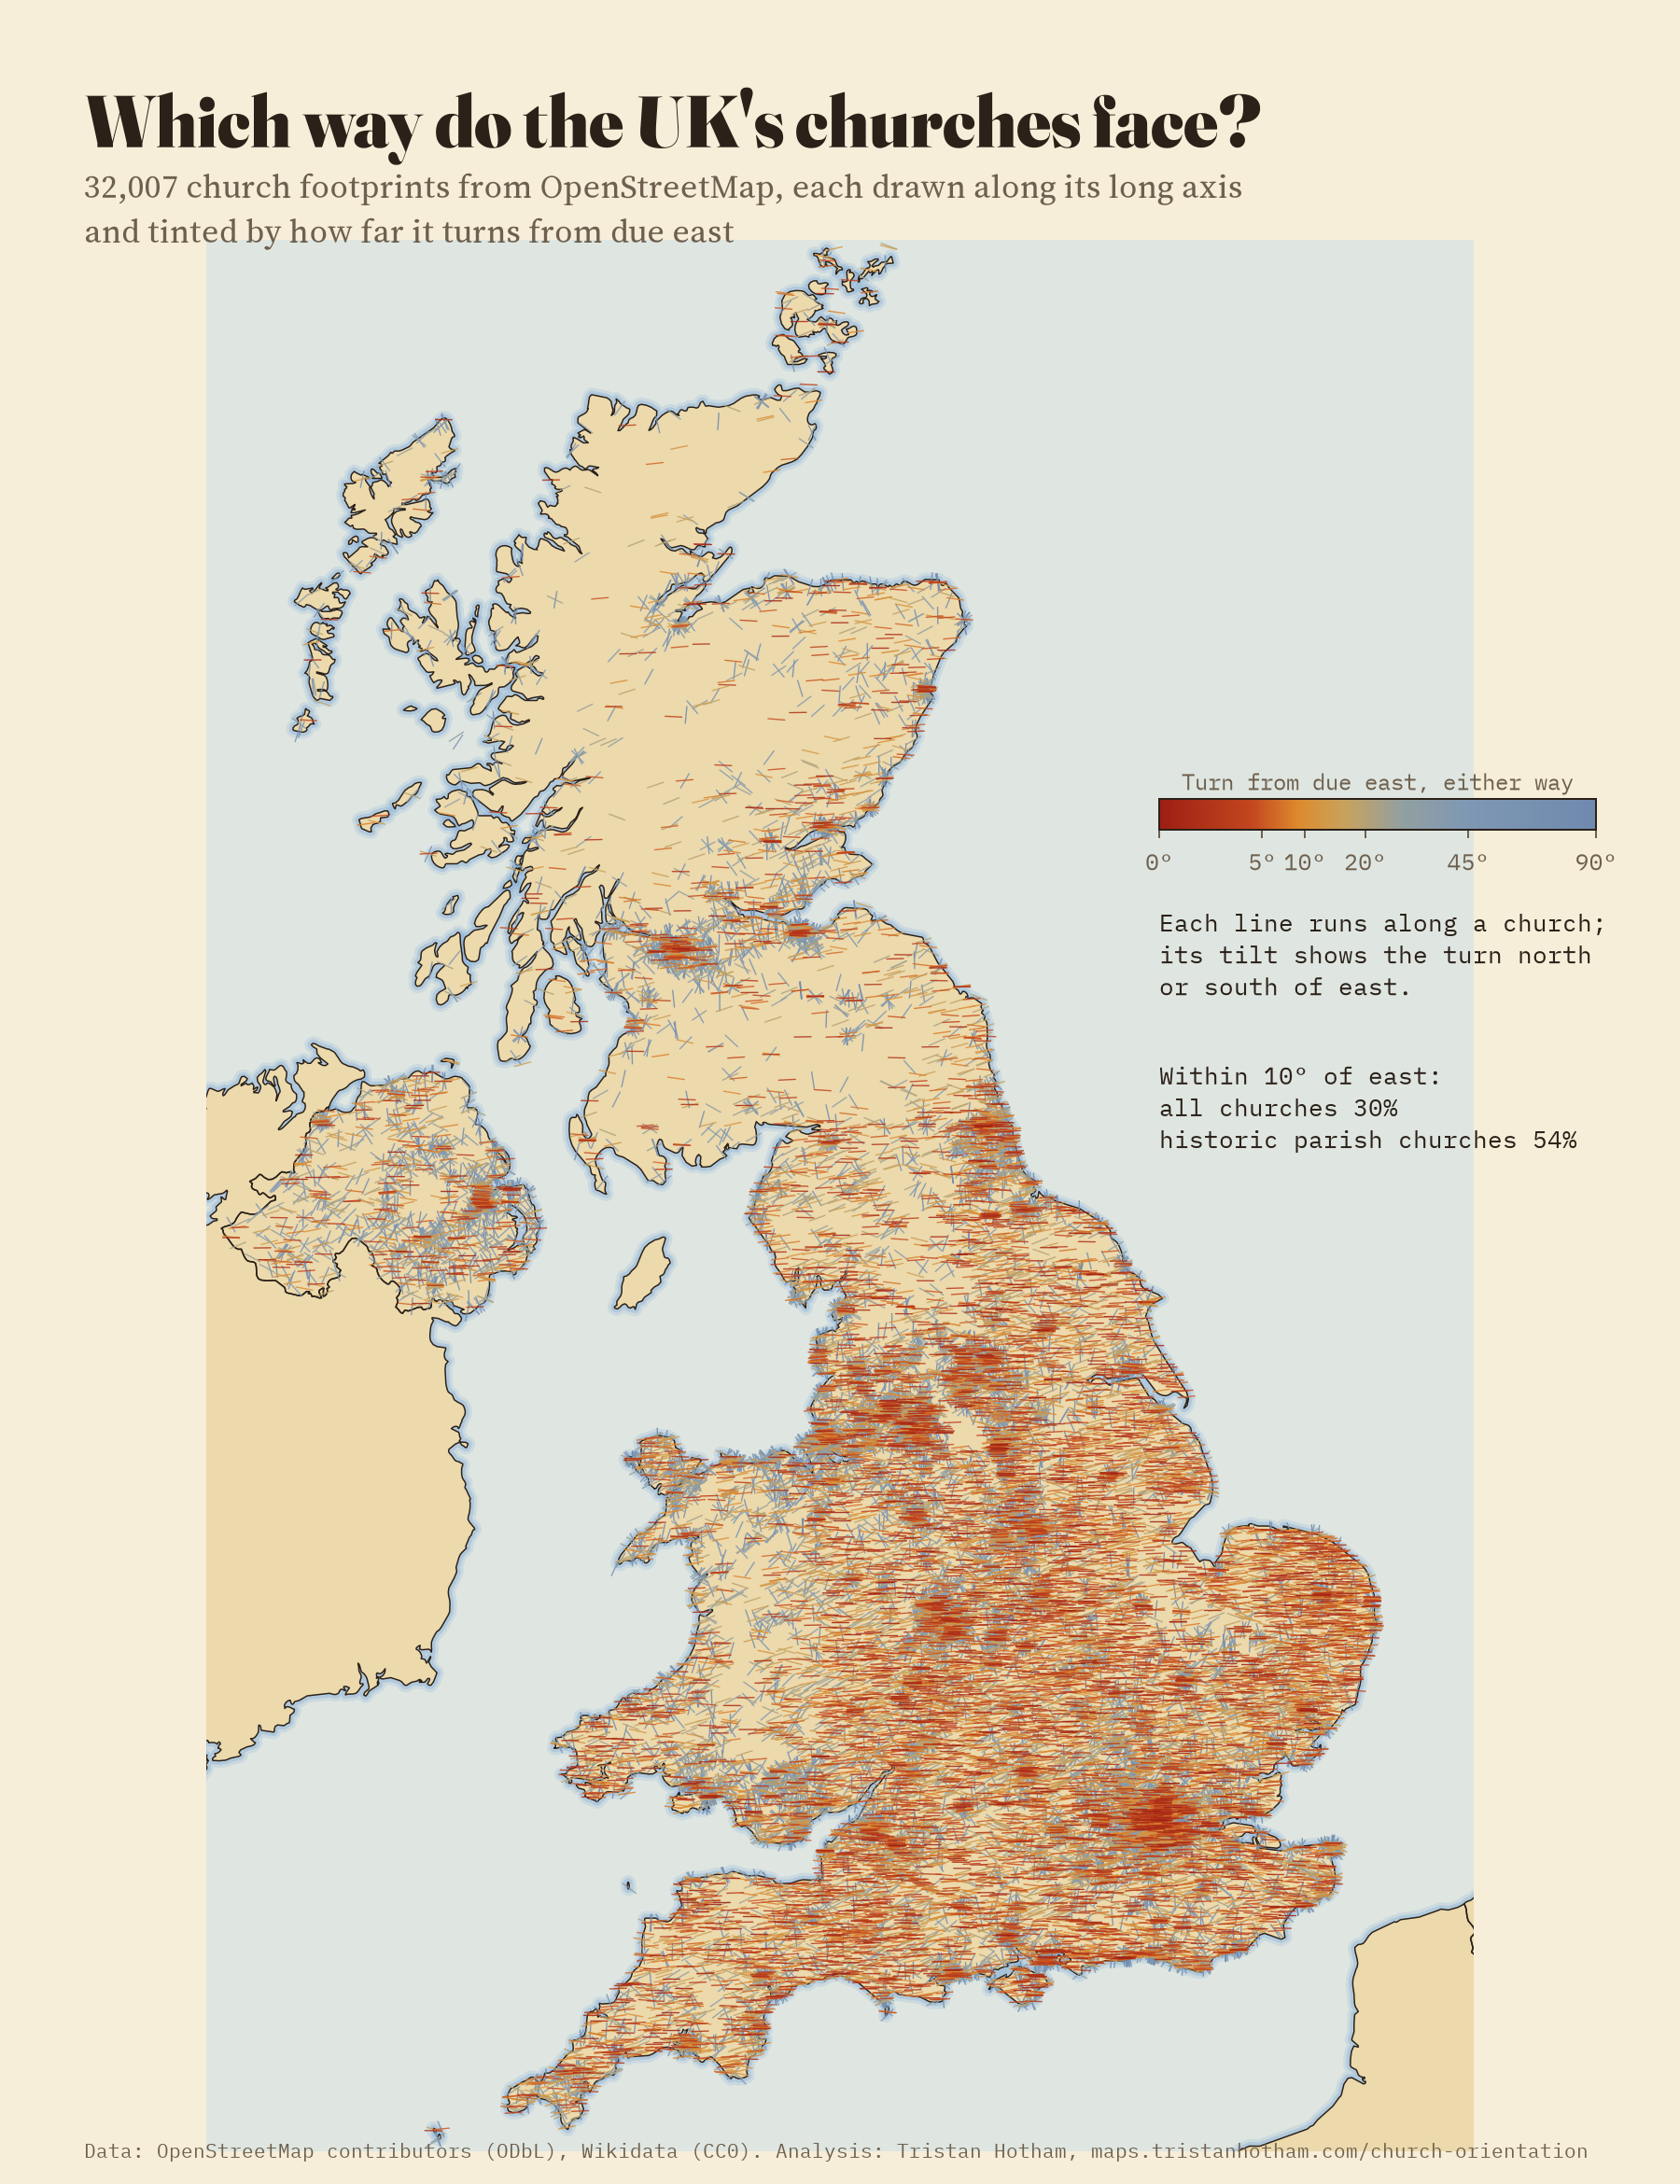
\includegraphics[width=0.86\textwidth]{f_map.png}
\caption{Every measured church as a short line along its axis, coloured by the size of its turn from due east.}\label{fig:map}\end{figure}

\subsection{Age, listing and denomination}
Age is the strongest divide (Figures~\ref{fig:roses} and \ref{fig:groups}; Table~\ref{tab:groups}). Of the historic parish churches, 53.5\% lie within 10° of east and 1.7\% beyond 45°, with a median deviation of 9.2°. Churches dated before 1540 are similar (55.1\% within 10°); those dated 1540 to 1799 reach 45.2\%, 1800 to 1913 24.9\% and 1914 onwards 19.9\%. Listing tells the same story: 53.8\% of Grade I churches, 50.6\% of Grade II*, 33.2\% of Grade II and 19.8\% of churches with no listing found. Anglican churches (44.8\%) are far more often east-facing than Roman Catholic (17.0\%), Church of Scotland (19.0\%) or Free Church buildings (14.2\%); the last is barely above the 11.1\% expected from random directions. Among churches dated 1800 onwards, Anglican churches still reach 32.7\%, against 17.5\% for Roman Catholic ones.

\begin{figure}[tbp]\centering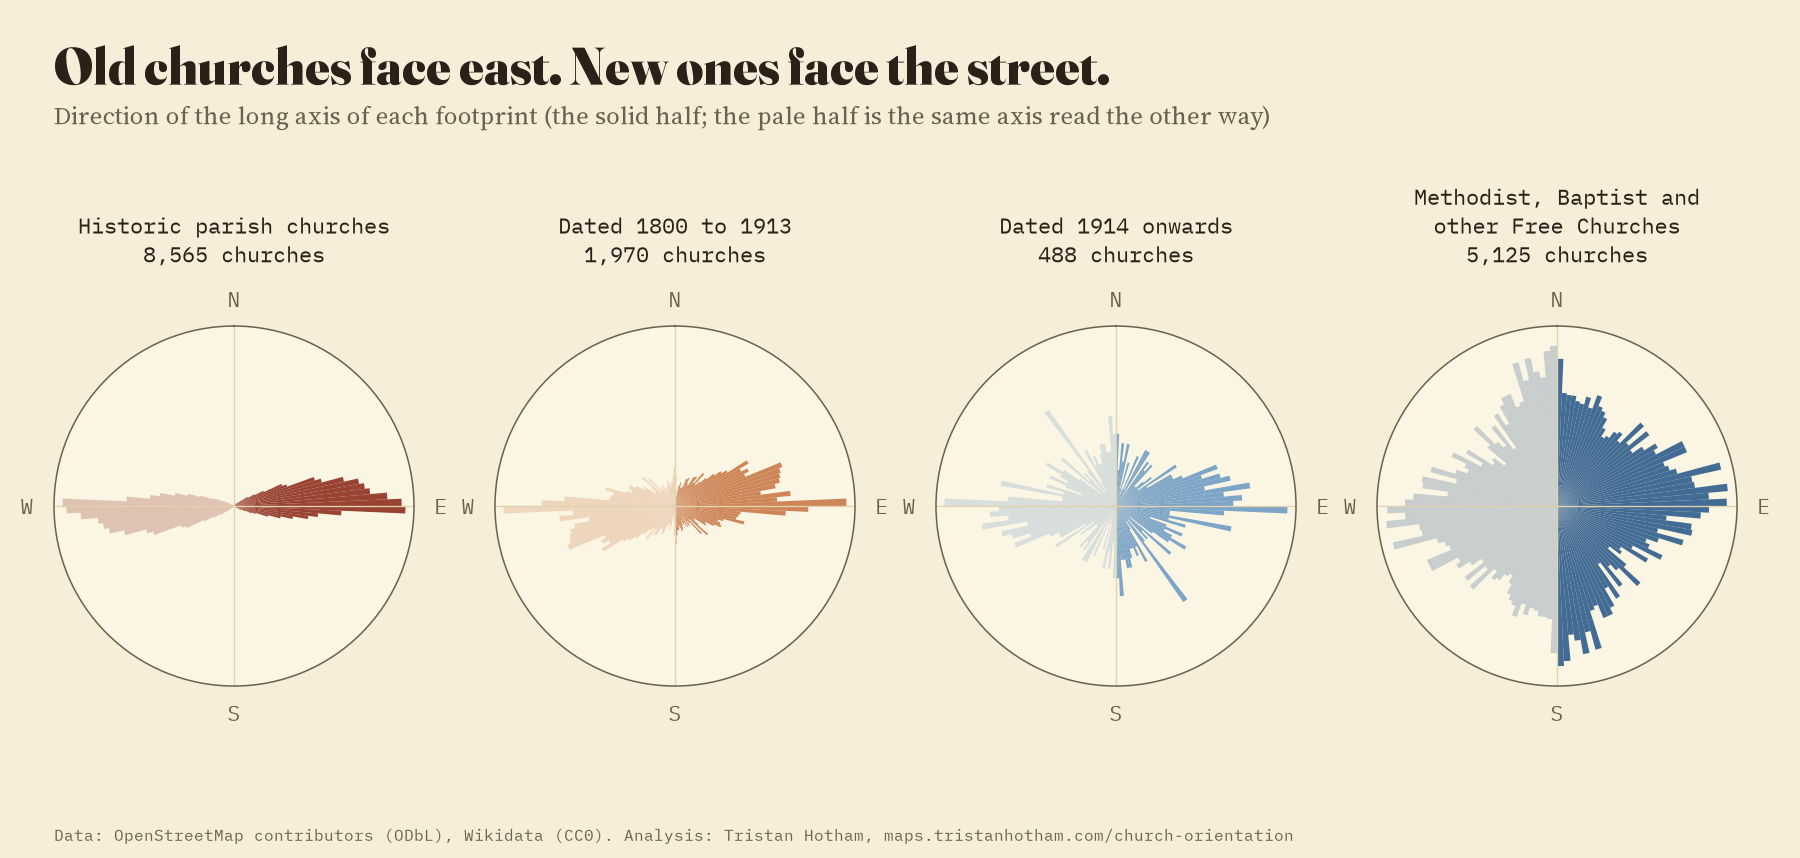
\includegraphics[width=\textwidth]{f_roses.png}
\caption{Rose diagrams of church axes for four groups.}\label{fig:roses}\end{figure}
\begin{figure}[tbp]\centering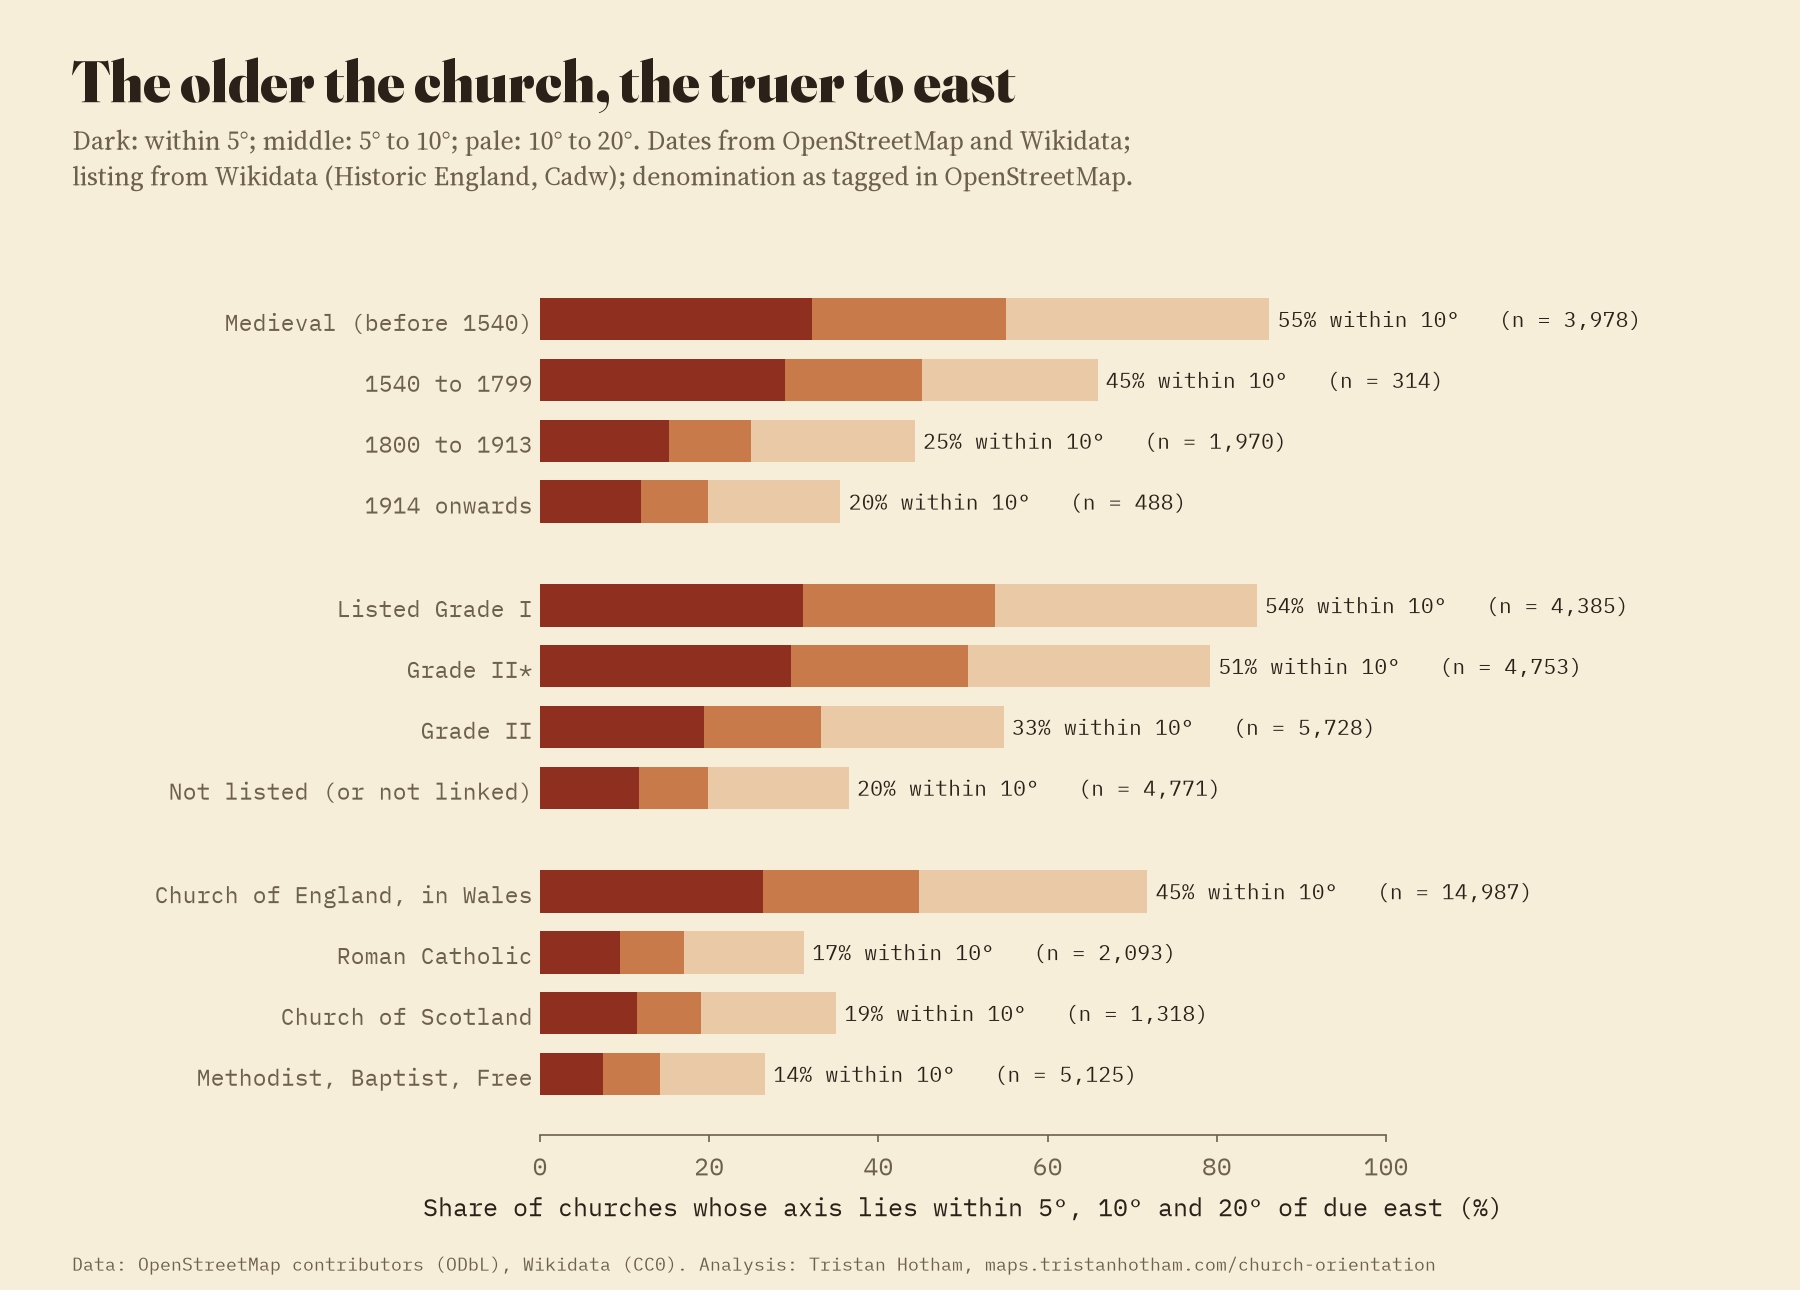
\includegraphics[width=0.92\textwidth]{f_groups.png}
\caption{Share of churches within 5°, 10° and 20° of due east by date, listing grade and denomination.}\label{fig:groups}\end{figure}

\begin{table}[tbp]\centering\small\caption{Share of churches (\%) within 5°, 10° and 20° of due east and beyond 45°, and the median absolute deviation (degrees), by group.}\label{tab:groups}
\begin{tabular}{lrrrrrr}\toprule Group & n & $\le$5° & $\le$10° & $\le$20° & $>$45° & Median\\
All measured & 32,007 & 17.6 & 30.4 & 50.7 & 26.2 & 19.6\\
Historic parish churches & 8,565 & 31.2 & 53.5 & 83.7 & 1.7 & 9.2\\
\midrule\multicolumn{7}{l}{\textit{Date}}\\
Before 1540 & 3,978 & 32.1 & 55.1 & 86.2 & 0.6 & 8.8\\
1540 to 1799 & 314 & 29.0 & 45.2 & 65.9 & 13.7 & 13.0\\
1800 to 1913 & 1,970 & 15.2 & 24.9 & 44.3 & 25.6 & 23.2\\
1914 onwards & 488 & 11.9 & 19.9 & 35.5 & 39.3 & 31.9\\
Not known & 25,257 & 15.5 & 27.0 & 45.7 & 30.2 & 23.0\\
\midrule\multicolumn{7}{l}{\textit{Listing}}\\
Grade I & 4,385 & 31.1 & 53.8 & 84.7 & 1.4 & 9.1\\
Grade II* & 4,753 & 29.7 & 50.6 & 79.2 & 4.1 & 9.9\\
Grade II & 5,728 & 19.4 & 33.2 & 54.8 & 18.9 & 17.5\\
Category A & 236 & 20.3 & 33.5 & 52.5 & 18.6 & 18.0\\
Category B & 881 & 14.9 & 25.1 & 42.8 & 32.6 & 25.3\\
Category C & 294 & 9.9 & 21.1 & 37.4 & 37.8 & 29.0\\
None found & 4,771 & 11.7 & 19.8 & 36.5 & 35.7 & 30.3\\
\midrule\multicolumn{7}{l}{\textit{Denomination}}\\
Church of England, in Wales, Episcopal & 14,987 & 26.4 & 44.8 & 71.8 & 8.0 & 11.6\\
Roman Catholic & 2,093 & 9.5 & 17.0 & 31.2 & 41.9 & 36.0\\
Church of Scotland and Presbyterian & 1,318 & 11.5 & 19.0 & 35.0 & 39.2 & 34.2\\
Methodist, Baptist and other Free Churches & 5,125 & 7.5 & 14.2 & 26.6 & 48.4 & 43.5\\
Orthodox & 83 & 16.9 & 21.7 & 43.4 & 34.9 & 28.1\\
Other Christian & 1,417 & 8.3 & 15.9 & 28.1 & 47.6 & 43.3\\
Not tagged & 6,984 & 11.6 & 20.7 & 36.4 & 37.5 & 30.8\\
\midrule\multicolumn{7}{l}{\textit{Nation}}\\
England & 25,121 & 19.1 & 32.9 & 54.3 & 23.7 & 17.6\\
Wales & 2,635 & 12.7 & 22.3 & 40.6 & 31.5 & 26.4\\
Scotland & 2,733 & 12.5 & 21.6 & 37.4 & 37.0 & 30.4\\
Northern Ireland & 1,518 & 10.7 & 19.2 & 32.5 & 39.7 & 34.3\\
\bottomrule\end{tabular}\end{table}

\subsection{The patron saint's day}
The feast-day hypothesis fails (Table~\ref{tab:feast}). For the 5,687 historic churches with a fixed-feast saint (66 saints), the mean absolute difference between axis and feast-day sunrise is 30.87°; with the saints shuffled it is 30.86° on average, so p = 0.54. Only 3.1\% of these churches lie within 3° of their feast-day sunrise, against 3.2\% under shuffling. The same holds for churches dated before 1540 (p = 0.72), for all churches (p = 0.82) and for churches dated 1800 onwards (p = 0.99). For comparison, the mean absolute difference from due east is 11.2° for the historic churches.

\begin{table}[tbp]\centering\small\caption{The feast-day test: mean absolute difference (degrees) between axis and feast-day sunrise for the real saints and, on average, for 10,000 random shuffles of the saints; one-sided p-value; and the share of churches (\%) within 3° of the predicted sunrise.}\label{tab:feast}
\begin{tabular}{lrrrrrrr}\toprule Churches & n & Saints & Real & Shuffled & p & $\le$3° real & $\le$3° shuffled\\\midrule
Historic parish churches & 5,687 & 66 & 30.87 & 30.86 & 0.54 & 3.1 & 3.2\\
Dated before 1540 & 2,626 & 62 & 31.10 & 30.96 & 0.72 & 3.0 & 2.9\\
Dated 1800 onwards & 941 & 61 & 39.44 & 37.71 & 0.99 & 4.8 & 5.0\\
All churches & 11,582 & 68 & 34.47 & 34.32 & 0.82 & 3.7 & 4.0\\
\bottomrule\end{tabular}\end{table}

Saint by saint (Figure~\ref{fig:saints}), the predicted sunrise ranges over 80.3° (from 49.4° to 129.7°), but the mean axes of the 32 saints' churches span only 7.8°, and the weighted regression slope of mean axis on predicted sunrise is -0.00. Historic churches of midsummer saints (John the Baptist, Peter, Peter and Paul, Botolph, Alban, Etheldreda, Barnabas; n = 1,281) have a mean axis of 85.5°, those of midwinter saints (Thomas, Thomas Becket, Nicholas, John the Evangelist, Stephen, Andrew, Edmund, Catherine, Clement; n = 1,073) 85.4°, a difference of -0.1° (Welch t test p = 0.79) where the hypothesis predicts 78.3°. Mary's 1,578 historic churches have a mean axis of 85.1°, indistinguishable from all historic churches (85.1°); this lies near the sunrise of the Annunciation (83.0°) and her Nativity (84.6°) but not of the Purification (114.7°) or Assumption (70.2°), and it cannot distinguish them from a general eastern habit.

\begin{figure}[tbp]\centering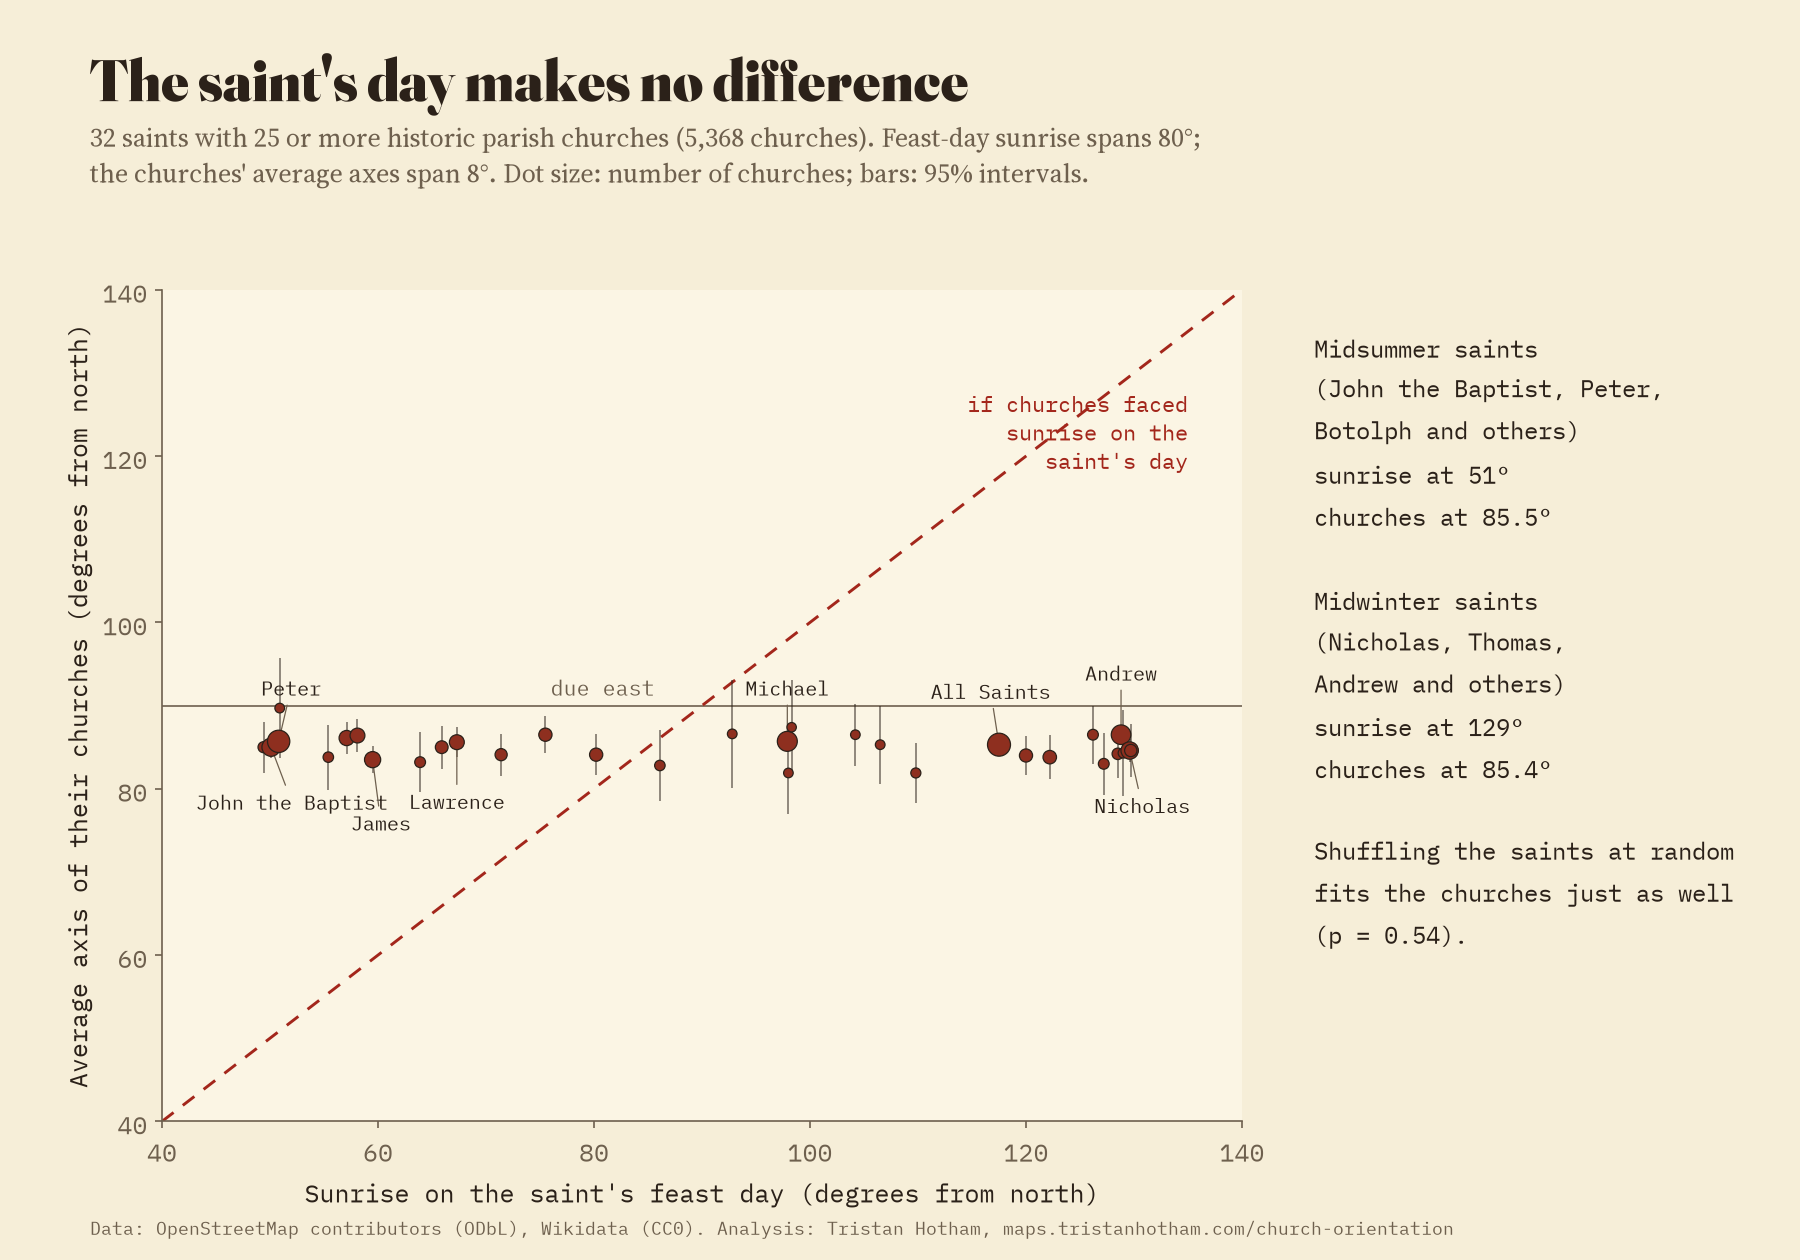
\includegraphics[width=0.92\textwidth]{f_saints.png}
\caption{Mean axis of each saint's historic parish churches against the sunrise on the saint's feast day (Julian dates moved to the solar year of foundation).}\label{fig:saints}\end{figure}

\subsection{A lean north of east, stronger in the west}
Historic churches within 45° of east turn north of it in 64.9\% of cases, with a mean deviation of -4.9° and a mean axis of 85.1°. The lean varies with longitude (Figure~\ref{fig:longitude}): in England and Wales, historic churches west of 3°W average -6.3° (n = 1,104), those east of the Greenwich meridian -2.1° (n = 2,023), and those east of 1°E 0.3° (n = 774); the linear slope is 0.94° per degree of longitude (r = 0.12). The direction matches \citet{hinton}, though the size of the difference here is smaller than his 10°.

\begin{figure}[tbp]\centering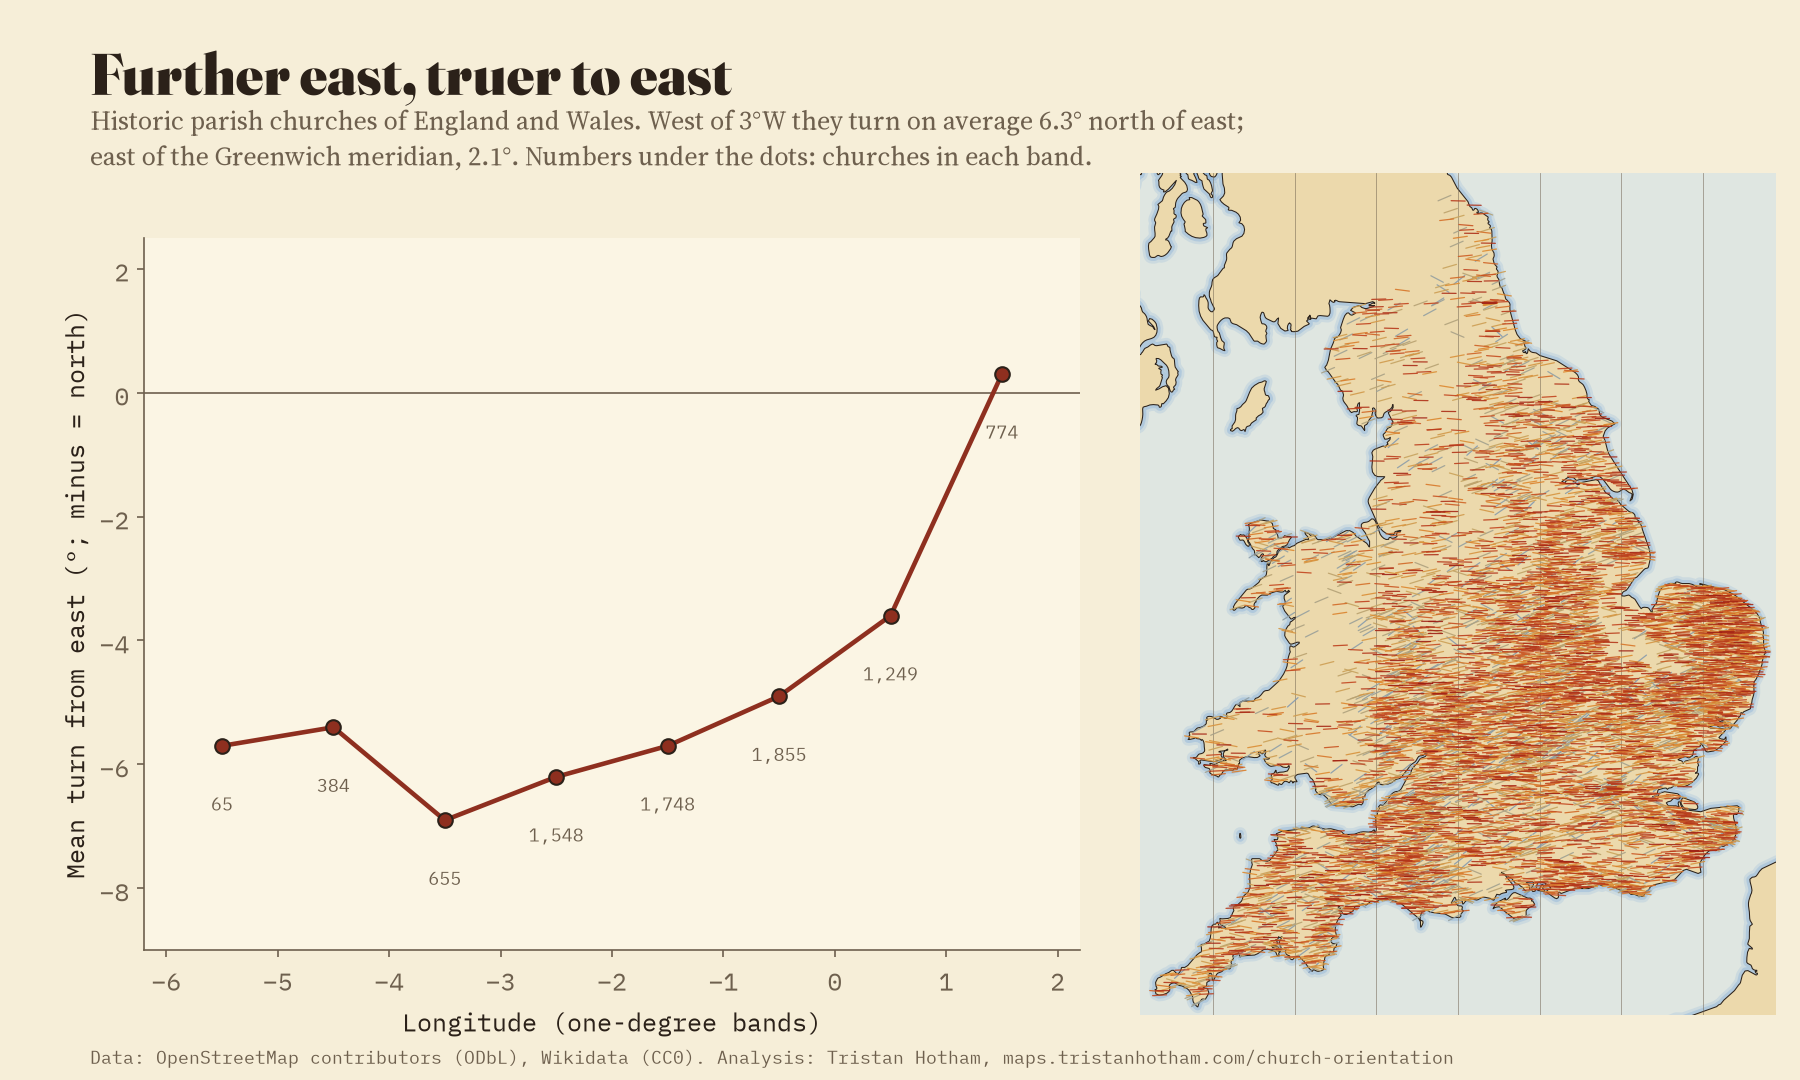
\includegraphics[width=\textwidth]{f_longitude.png}
\caption{Mean deviation of historic parish churches in England and Wales by one-degree band of longitude.}\label{fig:longitude}\end{figure}

\subsection{The street grid}
In the street sample (Figure~\ref{fig:streets}), urban churches dated 1800 onwards are closer to their street grid than to east in 84.5\% of cases where the two differ by at least 15° (n = 110), against 58.9\% for historic parish churches in towns (n = 73) and 89.5\% for urban Roman Catholic and Free Church buildings (n = 381). Among all urban churches in the sample, the median angle to the grid is 5.5° and to east 18.4°; among rural churches, 8.5° and 13.1°. Rural churches, too, are closer to their nearest roads than to east in 61.8\% of such cases, so the association runs both ways: later churches were fitted to existing streets, while lanes and streets were often laid out along an older churchyard. The grid is therefore a plausible cause of orientation only for later churches, and the historic urban sample is small. Figure~\ref{fig:footprints} shows five measured footprints.

\begin{figure}[tbp]\centering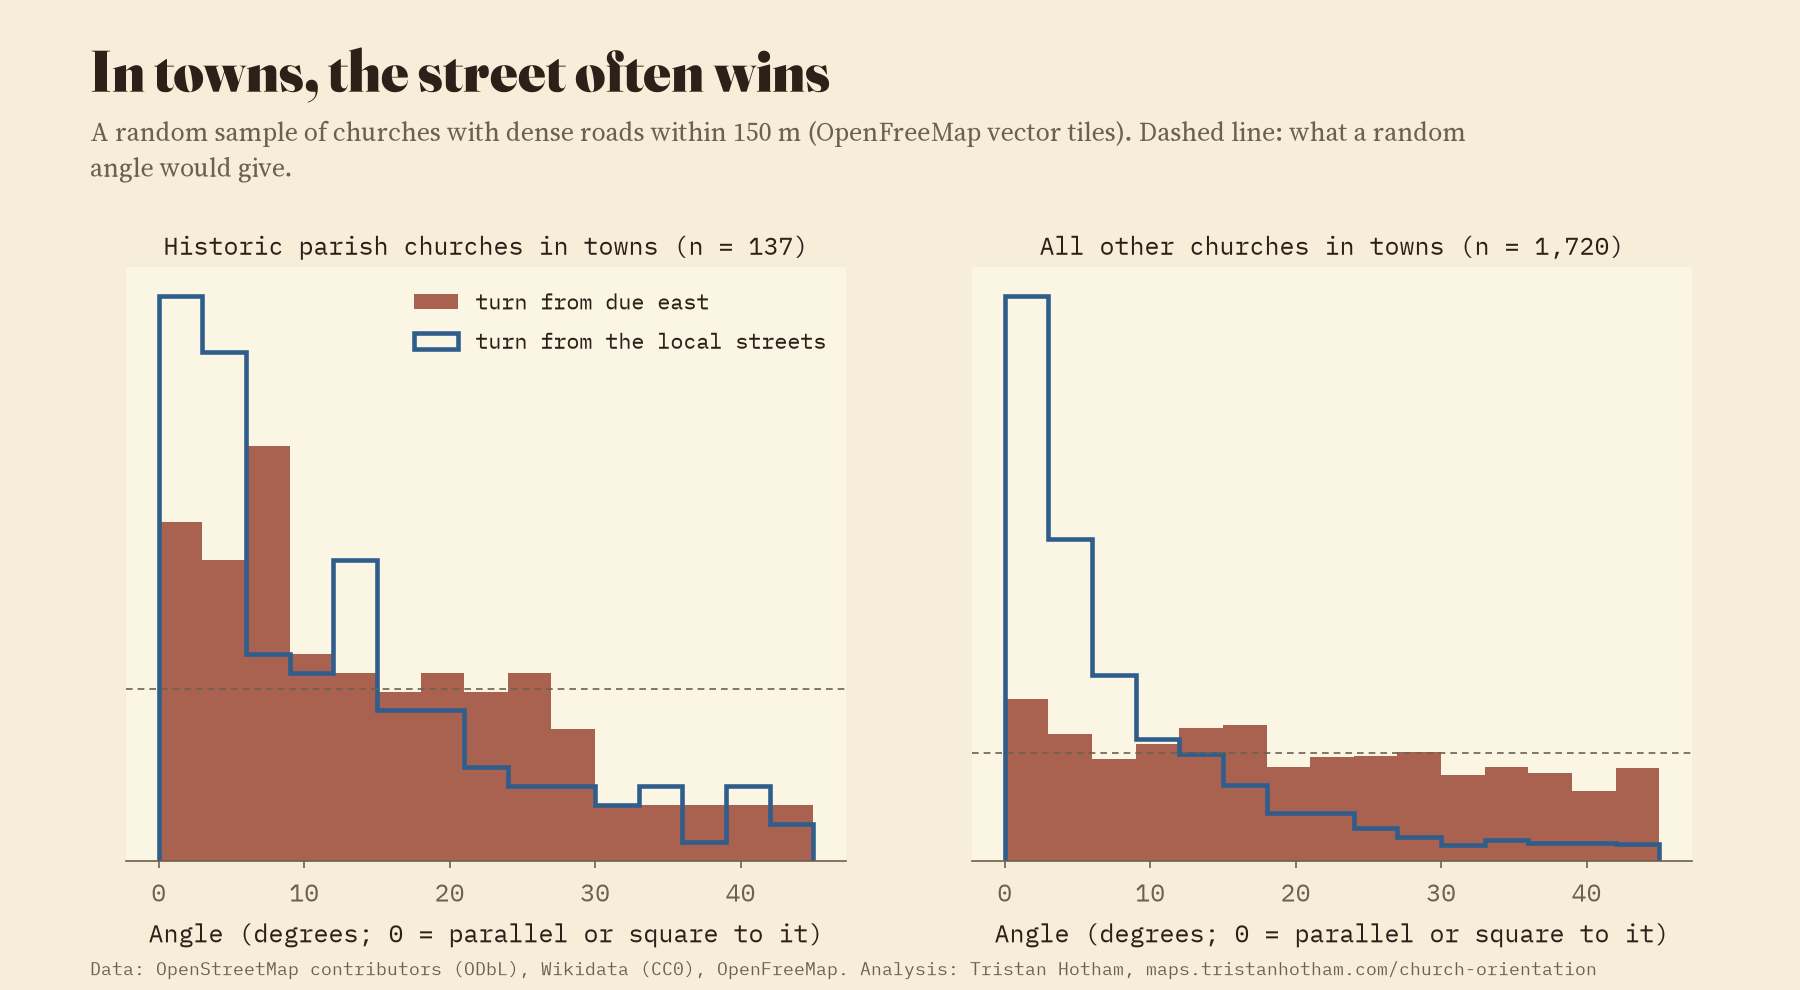
\includegraphics[width=\textwidth]{f_streets.png}
\caption{Angle of town churches to east (bars) and to the local street grid (line), folded to 0° to 45°.}\label{fig:streets}\end{figure}
\begin{figure}[tbp]\centering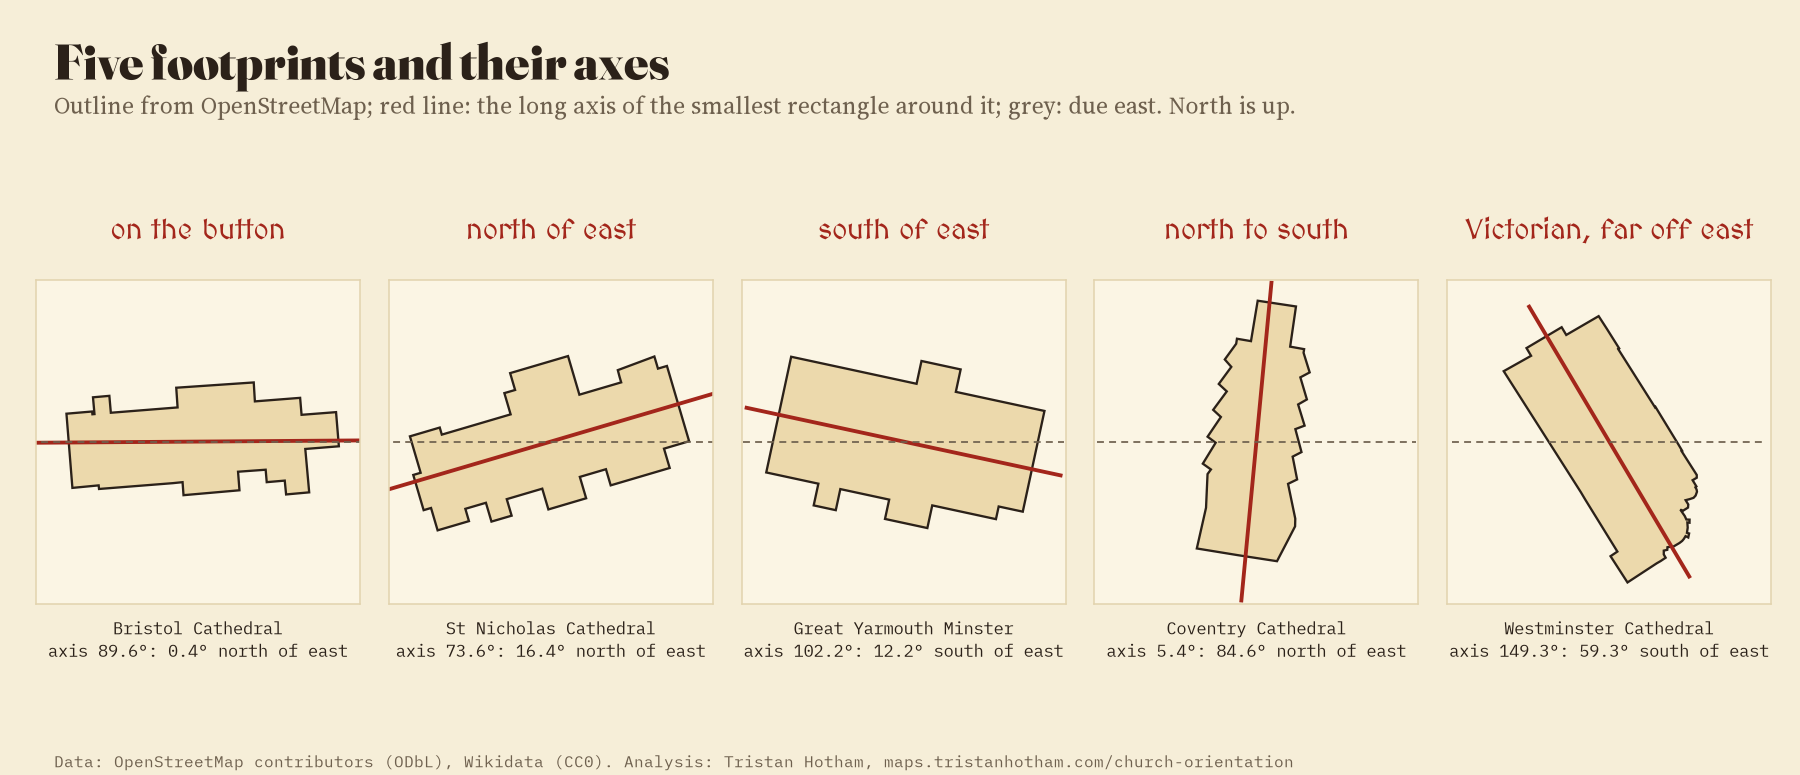
\includegraphics[width=\textwidth]{f_footprints.png}
\caption{Five footprints and their measured axes.}\label{fig:footprints}\end{figure}

\section{Limitations}
The footprint is not the nave. Towers, aisles, transepts, porches and later additions change the enclosing rectangle; for most parish churches the nave and chancel dominate the long axis, but a church whose chancel is set at an angle to its nave (a well-known feature of some churches) is reduced to one compromise axis, and a tower-heavy or cruciform plan can mislead. Mapping quality varies, and some outlines are traced roughly. Dates are sparse and uneven: Wikidata inception can be the foundation of a parish or an earlier church on the site rather than the standing building (Coventry Cathedral, rebuilt on a north to south axis in the twentieth century, carries the inception of its medieval predecessor), and the historic group relies partly on listing grade as a proxy for age. Dedications change over centuries, and the dedication recorded today may not be the one at foundation; many saints have several feasts, and the assumed foundation date for undated churches sets the calendar shift. The horizon is taken as flat; local hills delay sunrise and move its azimuth south, which matters most in the uplands. The street test uses the modern road network and a fixed radius. Finally, a null result for the patron-saint hypothesis does not explain the lean north of east; equinoctial or Easter sunrises, sightings by eye, or local custom all remain possible and cannot be separated with these data.

\section{Conclusion}
Most historic churches in the UK face within ten degrees of east, later churches much less so, and Free Church chapels almost at random. Whatever set the small turns of the old churches, it was not the sunrise on the patron saint's day: midsummer and midwinter saints face the same way, and the real saints fit the churches no better than shuffled ones. The old churches share a slight lean north of east, larger in the west, while many Victorian and later churches in towns follow their street.

\section*{Data and code availability}
The interactive map is at \url{https://maps.tristanhotham.com/church-orientation/}. Data and code are at \url{https://github.com/Tristan-Hotham/church-orientation} and archived with this paper at \url{https://doi.org/10.5281/zenodo.24052501}. The church table is derived from OpenStreetMap and released under the Open Database Licence; Wikidata is CC0; code is MIT licensed; text and figures CC BY 4.0.

\section*{AI statement}
I wrote the text, with drafting and editing assistance from Claude (Anthropic), which also helped prepare the analysis code. I reviewed and checked all text and results.

\begin{thebibliography}{99}
\bibitem[Ali and Cunich(2001)]{alicunich} Ali, J. R. and Cunich, P. (2001) The orientation of churches: some new evidence. \textit{The Antiquaries Journal} 81, 155 to 193. \url{https://doi.org/10.1017/S0003581500072188}
\bibitem[Bast and Buchhold(2017)]{qlever} Bast, H. and Buchhold, B. (2017) QLever: a query engine for efficient SPARQL+text search. In \textit{Proceedings of the 2017 ACM Conference on Information and Knowledge Management (CIKM)}, 647 to 656.
\bibitem[Freeman and Shapira(1975)]{freeman} Freeman, H. and Shapira, R. (1975) Determining the minimum-area encasing rectangle for an arbitrary closed curve. \textit{Communications of the ACM} 18(7), 409 to 413.
\bibitem[Furuhashi and Terado(2026)]{furuhashi} Furuhashi, T. and Terado, H. (2026) Between sacred tradition and urban form: an OpenStreetMap-based analysis of church orientation patterns in Milan. \textit{The International Archives of the Photogrammetry, Remote Sensing and Spatial Information Sciences} L-4/W1-2026, 43 to 48. \url{https://doi.org/10.5194/isprs-archives-L-4-W1-2026-43-2026}
\bibitem[Hinton(2006)]{hinton} Hinton, I. (2006) Church alignment and patronal saint's days. \textit{The Antiquaries Journal} 86, 206 to 226. \url{https://doi.org/10.1017/S0003581500000111}
\bibitem[Hotham(2026)]{saintsgeo} Hotham, T. (2026) The geography of saints. \url{https://github.com/Tristan-Hotham/saints-geography}
\bibitem[OpenFreeMap(2026)]{ofm} OpenFreeMap (2026) Free vector tiles (OpenMapTiles schema) from OpenStreetMap data. \url{https://openfreemap.org/}
\bibitem[OpenStreetMap contributors(2026)]{osm} OpenStreetMap contributors (2026) OpenStreetMap. Open Database Licence. \url{https://www.openstreetmap.org/}
\bibitem[Spencer(1971)]{spencer} Spencer, J. W. (1971) Fourier series representation of the position of the sun. \textit{Search} 2(5), 172.
\bibitem[Wikidata(2026)]{wikidata} Wikidata contributors (2026) Wikidata. CC0. \url{https://www.wikidata.org/}
\end{thebibliography}

\appendix
\section{Saint by saint}
\begin{longtable}{lrrrrrr}\caption{Saints with 25 or more historic parish churches: predicted feast-day sunrise (degrees from north) with the date as written and moved to the solar year of foundation, and the mean axis of their churches with its standard error.}\label{tab:saints}\\
\toprule Saint & Feast & n & Sunrise (as written) & Sunrise (Julian) & Mean axis & s.e.\\\midrule\endhead
Botolph & 17 Jun & 49 & 49.5 & 49.4 & 85.0 & 1.56\\
John the Baptist & 24 Jun & 371 & 49.6 & 50.1 & 85.0 & 0.68\\
Peter & 29 Jun & 823 & 49.8 & 50.8 & 85.7 & 0.45\\
Peter and Paul & 29 Jun & 29 & 49.9 & 50.9 & 89.7 & 3.09\\
Swithun & 15 Jul & 40 & 53.1 & 55.4 & 83.8 & 1.99\\
Margaret & 20 Jul & 177 & 54.4 & 57.1 & 86.1 & 0.97\\
Mary Magdalene & 22 Jul & 161 & 55.3 & 58.1 & 86.4 & 1.00\\
James & 25 Jul & 227 & 56.5 & 59.5 & 83.5 & 0.82\\
Oswald & 5 Aug & 45 & 60.1 & 63.9 & 83.2 & 1.82\\
George & 23 Apr & 87 & 69.9 & 65.9 & 85.0 & 1.31\\
Lawrence & 10 Aug & 163 & 63.6 & 67.3 & 85.6 & 0.93\\
Helen & 18 Aug & 72 & 67.4 & 71.4 & 84.1 & 1.29\\
Bartholomew & 24 Aug & 102 & 71.3 & 75.5 & 86.5 & 1.13\\
Giles & 1 Sep & 101 & 75.9 & 80.2 & 84.1 & 1.26\\
Cuthbert & 20 Mar & 40 & 90.8 & 86.1 & 82.8 & 2.19\\
Matthew & 21 Sep & 29 & 88.3 & 92.8 & 86.6 & 3.31\\
Michael & 29 Sep & 527 & 93.4 & 97.9 & 85.7 & 0.58\\
Chad & 2 Mar & 28 & 102.5 & 98.0 & 81.9 & 2.54\\
David & 1 Mar & 26 & 102.8 & 98.3 & 87.4 & 2.92\\
Denys & 9 Oct & 28 & 99.7 & 104.2 & 86.5 & 1.91\\
Wilfrid & 12 Oct & 29 & 101.9 & 106.5 & 85.3 & 2.40\\
Luke & 18 Oct & 34 & 105.4 & 109.8 & 81.9 & 1.86\\
All Saints & 1 Nov & 926 & 113.7 & 117.5 & 85.3 & 0.41\\
Leonard & 6 Nov & 99 & 116.3 & 120.0 & 84.0 & 1.20\\
Martin & 11 Nov & 110 & 118.9 & 122.2 & 83.8 & 1.33\\
Edmund & 20 Nov & 45 & 123.4 & 126.2 & 86.5 & 1.78\\
Catherine & 25 Nov & 45 & 124.8 & 127.2 & 83.0 & 1.92\\
Thomas Becket & 29 Dec & 57 & 129.6 & 128.5 & 84.2 & 1.47\\
Andrew & 30 Nov & 485 & 126.9 & 128.8 & 86.5 & 0.57\\
Stephen & 26 Dec & 34 & 129.8 & 129.0 & 84.3 & 2.64\\
Nicholas & 6 Dec & 303 & 128.3 & 129.6 & 84.6 & 0.72\\
John the Evangelist & 27 Dec & 76 & 130.6 & 129.7 & 84.6 & 1.62\\
\bottomrule\end{longtable}

\end{document}
